One of the algorithm in meta reinforcement learning is the meta-gradient reinforcement learning introduced in \cite{meta-gradient} by Google DeepMind. The main idea of this algorithm is to update the meta-parameters $\eta$ to achieve a better learning performance. The details of this algorithm is presented in this section.

\par
In deep reinforcement learning, the environment model is often unknown to the agent. Therefore, the true value function has to be approximated by a function known as \textit{return} with parameter $\theta$. This return function plays an important role in determining the characteristics of the reinforcement learning algorithm. Usually, the return function is parameterised by a discount factor $\gamma$ and the bootstrapping parameter $\lambda$, which are denoted as meta-parameters $\eta$ in this paper. Throughout normal training process, these two parameters $\gamma$ and $\lambda$ are hand-selected and held fixed. Following are the \textit{n}-step return\cite{n-step-return} depending on fixed $\gamma$:

\[g_{\eta}\left(\tau_{t}\right)=R_{t+1}+\gamma R_{t+2}+\ldots,+\gamma^{n-1} R_{t+n}+\gamma^{n} v_{\theta}\left(S_{t+n}\right)\]

where $\eta = \{\gamma\}$, \textit{t} is the current time step, and the $\lambda$ return\cite{lambda-return} depending on fixed $\gamma$ and $\lambda$:

\[g_{\eta}\left(\tau_{t}\right)=R_{t+1}+\gamma(1-\lambda) v_{\theta}\left(S_{t+1}\right)+\gamma \lambda g_{\eta}\left(\tau_{t+1}\right)\]

where $\eta = \{\gamma, \lambda\}$. In addition, the parameter $\theta$ is updated by the following formula, taking fixed $\eta$ into account:

\[\theta' = \theta + f(\tau, \theta, \eta)\]

where $\tau$ is the sample of experience being considered.

\par
In order to achieve better performance, the algorithm introduced in \cite{meta-gradient} updates $\eta$ during the training process. Besides an objective function $J(\tau, \theta, \eta)$, whose value the parameter $\theta$ is being updated to reduce, a meta-objective defined as $\bar{J}\left(\tau^{\prime}, \theta^{\prime}, \bar{\eta}\right)$ is also included into this algorithm and the purpose of updating $\eta$ is to increase its value.

\par
Here is how the algorithm works: First, the algorithm starts with parameter $\theta$ and applies the update function on the first sample, resulting in an updated parameter $\theta'$. After that, the performance is measured by $\bar{J}(\tau', \theta', \bar{\eta})$, where $\tau'$ is the next sample following $\tau$ and $\bar{\eta}$ is a fixed meta-parameter. Then, the gradient of the meta-objective with respect to the meta-parameters $\eta$ is obtained by applying the chain rule:

\[\frac{\partial \bar{J}\left(\tau^{\prime}, \theta^{\prime}, \bar{\eta}\right)}{\partial \eta}=\frac{\partial \bar{J}\left(\tau^{\prime}, \theta^{\prime}, \bar{\eta}\right)}{\partial \theta^{\prime}} \frac{\mathrm{d} \theta^{\prime}}{\mathrm{d} \eta}\]

The term $\frac{\mathrm{d} \theta^{\prime}}{\mathrm{d} \eta}$ can be calculated as follows:

\begin{align*}
	\frac{\mathrm{d} \theta^{\prime}}{\mathrm{d} \eta}&=\frac{\mathrm{d} \theta}{\mathrm{d} \eta}+\frac{\partial f(\tau, \theta, \eta)}{\partial \eta}+\frac{\partial f(\tau, \theta, \eta)}{\partial \theta} \frac{\mathrm{d} \theta}{\mathrm{d} \eta} \\
	&=\left(\mathrm{I}+\frac{\partial f(\tau, \theta, \eta)}{\partial \theta}\right) \frac{\mathrm{d} \theta}{\mathrm{d} \eta}+\frac{\partial f(\tau, \theta, \eta)}{\partial \eta}
\end{align*}

In practice, the gradient $\partial f(\tau, \theta, \eta) / \partial \theta$ is large and challenging to compute, because it is a N x N matrix, where N is the number of parameters in $\theta$. Therefore, a simple approximation is to set $\partial f(\tau, \theta, \eta) / \partial \theta=0$, which is especially cheap to compute. Finally, $\Delta\eta$ is calculated as follows to maximize the meta-objective:

\[\Delta \eta = -\beta \frac{\partial \bar{J}(\tau', \theta', \bar{\eta})}{\partial \theta'} \frac{\partial f(\tau, \theta, \eta)}{d\eta}\]

where $\beta$ is the learning rate for updating $\eta$.

\par
The validation of meta-gradient algorithm is executed on Arcade Learning Environment with an agent built with the IMPALA framework. The agents are evaluated on 57 different Atari games and the median of human-normalised scores are documented in the following table:
\begin{figure}[H]
	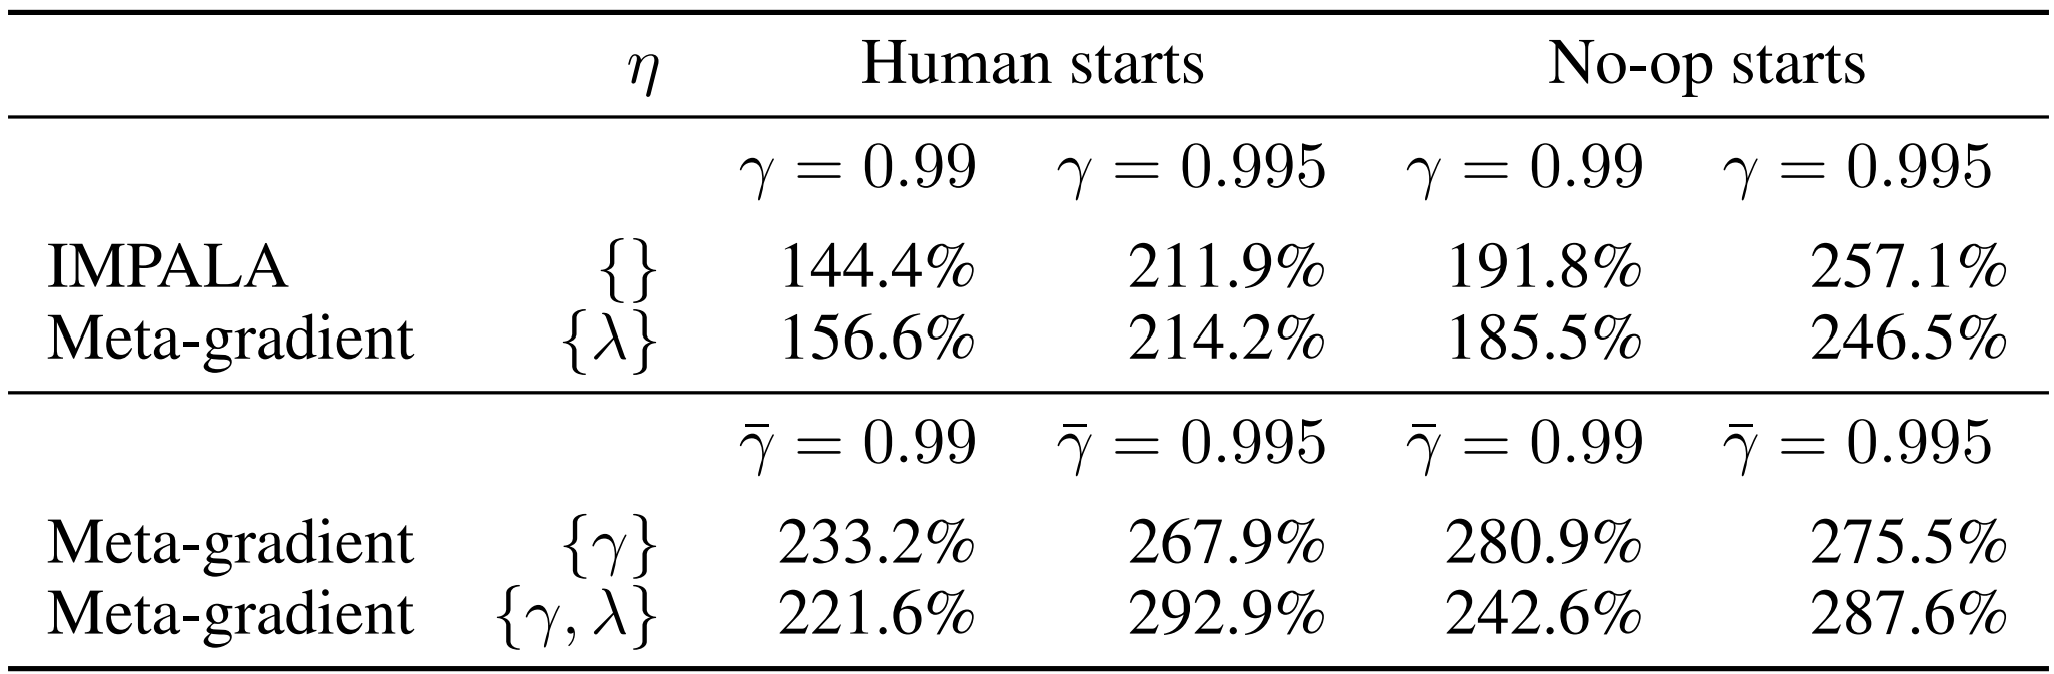
\includegraphics[scale=0.3]{meta-gradient-result.png}
	\centering
	\caption{Experiment result of meta-gradient algorithm. "Human starts" means episodes are initialized to a state that is randomly sampled from human play, while "No-op starts" means each episode is initialized with a random sequence of no-op actions.}
	\label{meta-gradient-result}
\end{figure}
We can see that meta-gradient algorithm has a better performance than the baseline IMPALA algorithm.
% 
% 
% 